\documentclass[a4paper, binding=0.6cm, noexaminfo, english]{sapthesis}

\usepackage{microtype}
\usepackage[english]{babel}
\usepackage[utf8]{inputenc}
\usepackage{hyperref}
\usepackage{framed}
\usepackage{listings}
\usepackage{xcolor}

\hypersetup{
	pdftitle={Data Leak Detection in Mobile Application},
	pdfauthor={Nicola Iommazzo}
}
\hypersetup{
    colorlinks,
    citecolor=black,
    filecolor=black,
    linkcolor=black,
    urlcolor=black
}

\lstdefinestyle{mystyle}{   
    backgroundcolor=\color{lightgray},
    breakatwhitespace=false,         
    breaklines=true,                 
    captionpos=b,                    
    keepspaces=true,                   
    numbersep=5pt,                  
    showspaces=false,                
    showstringspaces=false,
    showtabs=false,                  
    tabsize=2
}

\lstset{style=mystyle}

\title{Data Leak Detection in Mobile Applications}
\subtitle{Confidentiality of Personal Data}
\author{Iommazzo Nicola}
\IDnumber{1693395}
\course{Engineering in Computer Science}
\courseorganizer{Dipartimento di Ingegneria Informatica, Automatica e Gestionale}
\AcademicYear{2022/2023}
\advisor{Prof. Leonardo Querzoni}
\coadvisor{Pierluigi Pierini}
\coadvisor{Paolo Piccolo}
\thesistype{Master thesis}
\copyyear{2023}
\authoremail{iommazzo.1693395@studenti.uniroma1.it}

\begin{document}

	\frontmatter
	
		\maketitle
	
		\begin{acknowledgments}
	 Acknowledge n1
	\newline
	Acknowledge n2
	\newline
	\newline
	TODO: 
	\begin{itemize}
		\item Abstract
		\item App case: Radarbot
		\item App case: Waze
		\item App case: GoogleMaps
		\item Conclusion
	\end{itemize}
\end{acknowledgments}
		\begin{abstract}
	Briefly describe the whole content of the thesis.
\end{abstract}

		\tableofcontents

	\mainmatter
	
		\chapter{Introduction}
	
	\par Mobile applications are now part of our daily life. Everyone of us make use of different applications during their daily routine. There are applications for literally every kind of necessity: we would like to know what the weather will be like in the next days in our city, we would like to keep track of our fitness training that every morning we do in the neighbourhood, or we would like to know how the traffic is on the way back to our home. Using these applications is becoming a real habit, and like any other habit we do not ask ourselves anymore why are we doing it, or how are we doing it.
	\par Going through the years it is becoming much more common to hear about the terms \textit{data breaches} or \textit{data leak} on a multitude of online applications. The whole amount of data that users has put in their account can be exposed to leak of this kind. \newline
	Nowadays people tend to use applications without even realise the amount of informations they are delivering to the network, profile pictures, email addresses and phone numbers, and so on. All of these data are private informations, maybe the user does not like to share to everyone else, but just with the system on order to get the customized experience the application is offering. \newline 
	\par Mobile applications handle private data of millions of different users, therefore it is mandatory checking the robustness and any kind of protection implemented in the application, in order to make it resilient to possible leaks of user informations.
	
	\section{Personal Data}
		\par The concept of personal data is something I would like to make clear. There are multiple definitions and laws defining the scope of this kind of informations. As stated by the European Commission~\cite{European Commission}:
		\begin{framed}
			\textit{
				Personal data is any information that relates to an identified or identifiable living individual. Different pieces of information, which collected together can lead to the identification of a particular person, also contribute personal data. \newline
				\indent Personal data that has been de-identified, encrypted or pseudonymised but can be used to re-identify a person remains personal data and falls within the scope of the GDPR. [...] \newline
				\indent The GDPR protects personal data regardless of the technology used for processing that data - it is technology neutral and applies to both automated and manual processing. [...]
			}
		\end{framed}
		\par Practical examples of informations falling in the category of personal data are - name and surname, address, phone number, date of birth, but also photographs, ip addresses, location informations. \newline
		\par Dealing with mobile applications, personal informations are often typed in directly by the user, most likely at the moment of the creation of a new user profile, but not only. Some personal data might be shared automatically during the use of such application, like ip address or advertising phone identifier. \newline
		These information not necessarily are mandatory to access the services offered by the application. Personal data might contribute to some advertising service bundled within the application to keep track of the user data, or these data might be sent to some logging service implemented in the application in order to retrieve statistics on the users utilizing that application. 
	
	\section{Goals}
		\par Goal of the study in this thesis is to check if software features expose it to the risk of providing more information than planned. \newline
		A mobile application might share private informations with or without our accord in different moment while using it. For instance our contact list might be shared while using an application when synchronizing our friend list.
		\par Goal is therefore ensuring there is no leak of private data for the whole activity and at any moment for a specific application.
		\newline
		\par The work was conducted by examining applications running on Android operative system. Different mobile applications have been analyzed belonging to three different area of interests:
		\begin{itemize}
			\item \underline{Weather}: General applications \textit{without} user authentication.
			\item \underline{Health \& Fitness}: Applications \textit{with} user authentication and \textit{some} interaction between users.
			\item \underline{Maps \& Navigation}: Sophisticated applications  \textit{with} user authentication and \textit{continuous} interactions with server or other users.
		\end{itemize}
		\par The order in which the applications have been investigated has been decided basing on an increasing complexity and notoriety of them. Starting from weather forecast applications that generally do not require any kind of user authentication, going through fitness applications that let the user customize and share fitness routines to other users, and finally analyzing applications that manage geographical informations to retrieve real time traffic data.
		 
	\section{Methodologies}
		\par Since the goal is to detect any personal data leak while using the application, dynamic analysis is the main method used to investigate applications behaviour. In particular each mobile application has been inspected starting from the \textbf{network traffic analysis}, generated by the application at runtime. \newline
		Every action carried out by the user in the context of an application will generate some request to a server. Notice that mobile applications do not communicate only with the server offering that service. Indeed in the implementation of a mobile application there are different activities, each one provide a different service - for example advertisement services, logging services, push notification services, and so on. Every request is therefore generated by the application and might potentially include our personal data.		
		\par Where the network sniffing offered a spotlight for some in-depth study, a \textbf{static analysis} has been adopted going through an examination of the code of the application. Static analysis on an Android application is really dispersive and time consuming. An Android Package file (APK) can contain hundreds of thousands of Java classes. The majority of the compiled applications is stripped from the symbols, so methods and classes names cannot be directly found in the source code. Most of the time a simple obfuscation method like symbols stripping combined with the high number of classes, it is sufficient to hide something very interesting, for instance the method used to compute the \textit{Authorization header} in an HTTP request.
		\par To know more about the static and dynamic analysis tools I used in the practice, go to Chapter \ref{chap:testing_environment}.
				
	\section{Collaboration with IPS}
		\par Da definire ...


		\chapter{Fundamentals}
	\par This chapter is dedicated to illustrate some fundamental knowledge in order to fully understand the work I have done while investigating specific applications. Some of them are technologies arised in last ten years, improving not only the efficiency but also the stability and portability of the standard development of mobile applications. \newline
	Generally Android mobile applications are client implementations for specific services. The scenario is therefore the classic client-server communication model where each client interacts with one or more server. \newline
	\par First of all client and server must establish a connection between them, hopefully a \textit{secure connection}. This is the first topis explained in this section. Client and server, that means mobile application and application server, agree to find a secure way to communicate each other. 
	\par Once the connection is established there are lots of ways in which an application can send information. This is the problem of the data serialization. Informations can be represented using different Interface Description Languages (IDL). Starting from the classic JSON or XML format, passing through binary. Each representation has advantages and disadvantages. In particular there is a section dealing with an IDL that is widely used in mobile application, that is \textit{Protocol Buffer}.
	\par After having described the interation of a standard mobile application, there is a section explaining the concept of RPC, and in particular the recent developed \textit{gRPC} framework. As I said most of the mobile applications reflect the client-server paradigm. It is modern framework able to delegate some procedure in the client to the server, improving performance and portability of the application service.
	\par Finally the last section of this chapter deals with a new network procol called \textit{QUIC}, a modern evolution of the HTTP/2 protocol used by most of the recent applications.
		
	\section{HTTPS: HTTP over TLS}
		\par As stated in the online documentation for Android Developers~\cite{android_dev_tips} it is a good practice to protect applications data using the \textbf{Transport Layer Security (TLS)} along with the standard HTTP protocol. \newline
		TLS is a protocol designed to provide communications security over a computer network.  
		It provides \textit{confidentiality}, \textit{authentication} and \textit{integrity} meaning that: data is encrypted for third parties, ensure that both parties actually are who they pretend to be, ensure that data is not modified in the transit.
		\par A server (or web application) that wants to use TLS must have installed an \textbf{SSL certificate} on the machine. This certificate is released by a \textbf{Certificate Authority (CA)} for a specific domain, and contains important informations on the owner of that domain together with the public key of the server.  
		\par Every time a client wants to establish a connection with a server using TLS, the TLS Handshake procedure is issued.	
		\par There are also some mitigations Android mobile application developer can use in order to limitate authority checks
		
		\subsection{SSL/TLS Handshake}
			\par During the TLS handshake both mobile application and server exchange informations to set up a bidirectional encrypted connection. For this reason TLS version (1.0, 1.2, 1.3, etc) and cryptographic suite are agreed. Moreover the client verifies the authenticity of the server basing on its certificate. Finally both the endpoints will generate session keys to encrypt and decrypt the messages they will exchange each other. Once data are encrypted, they are signed with a Message Authentication Code (MAC), so that the receiver can verify the integrity of the data sent over the network.
			\begin{figure}[ht]
				\centering
				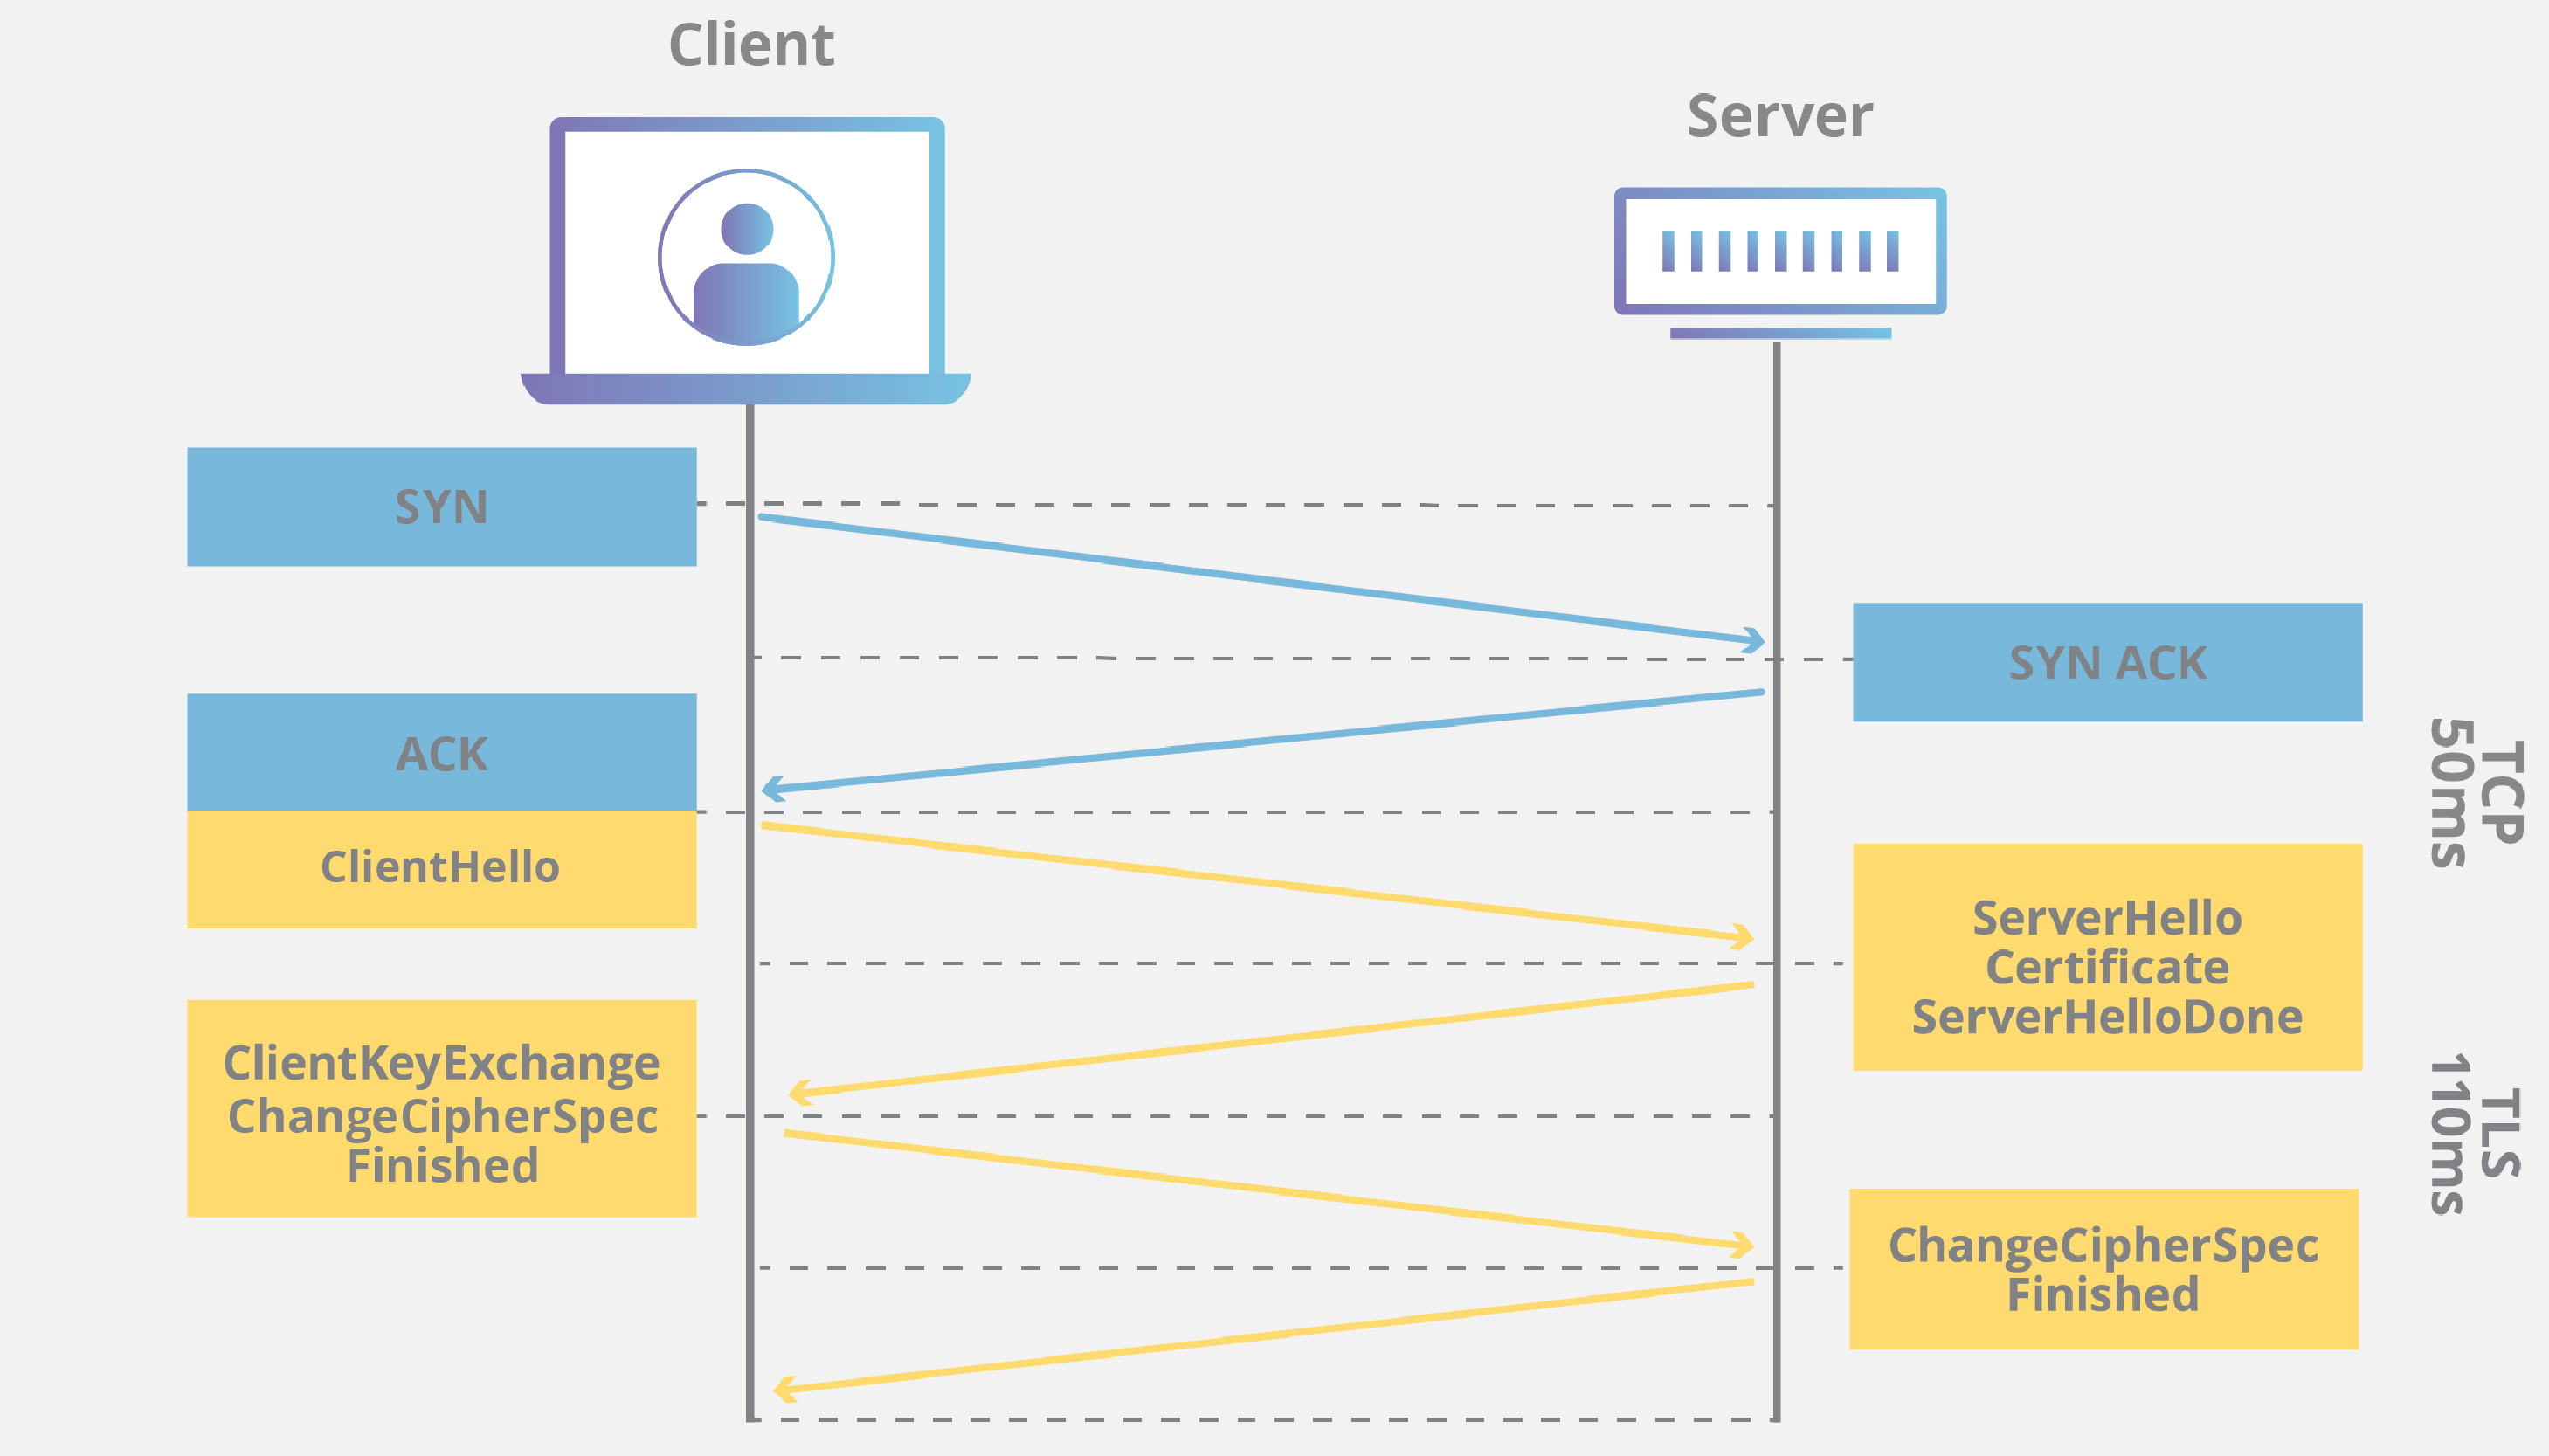
\includegraphics[width=0.8\textwidth]{images/tcp-tls-handshake.png}
				\caption{TCP Handshake and TLS Handshake communication flow needed to set up a secure connection. \cite{image_tcp_tls_handshake}}
				\label{fig:tcp_tls_handshake}
			\end{figure}
			\par From the performance point of view, the whole process of the TLS handshake needs both the endpoints to communicate before the data are actually transmitted over the network. In particular in the TLS versions < 1.3, two round trip time are needed to set up the whole connection \textit{(110ms)}. This amount of time added to the standard TCP three-way-handshake \textit{(50ms)} to establish the session between client and server, results in average in less then \textit{0.2 seconds} spent only to set up a secure connection without actually sending any application data yet. 
			\newline
 			As I said TLS makes possible to exchange information over a non-secure channel by providing confidentiality, authentication and integrity.  
			
		\subsection{Certificate Verification}
		\label{subsec:certificate_verification}
			\par A procedure I would like to stress is the certificate validation routine that happens at the really start of every TLS handshake. At the moment the client wants to establish a connection with the server, it needs the certificate to check the server is the actual endpoint the client want to talk with. The first thing the client does is to check that the certificate showed by the server is not expired, and that the server domain name matches with the one reported in the certificate. The next step performed by the client is to verify that the certificate has been signed by the certificate authority that authorized it. This procedure is done by verifying that the issuer's CA name matches the owner's CA name at the above level, and using the owner's CA signature and public key to verify the certificate is properly signed. The process is repeated until a CA trusted by the client is met, usually a root CA.
			\begin{figure}[ht]
				\centering
				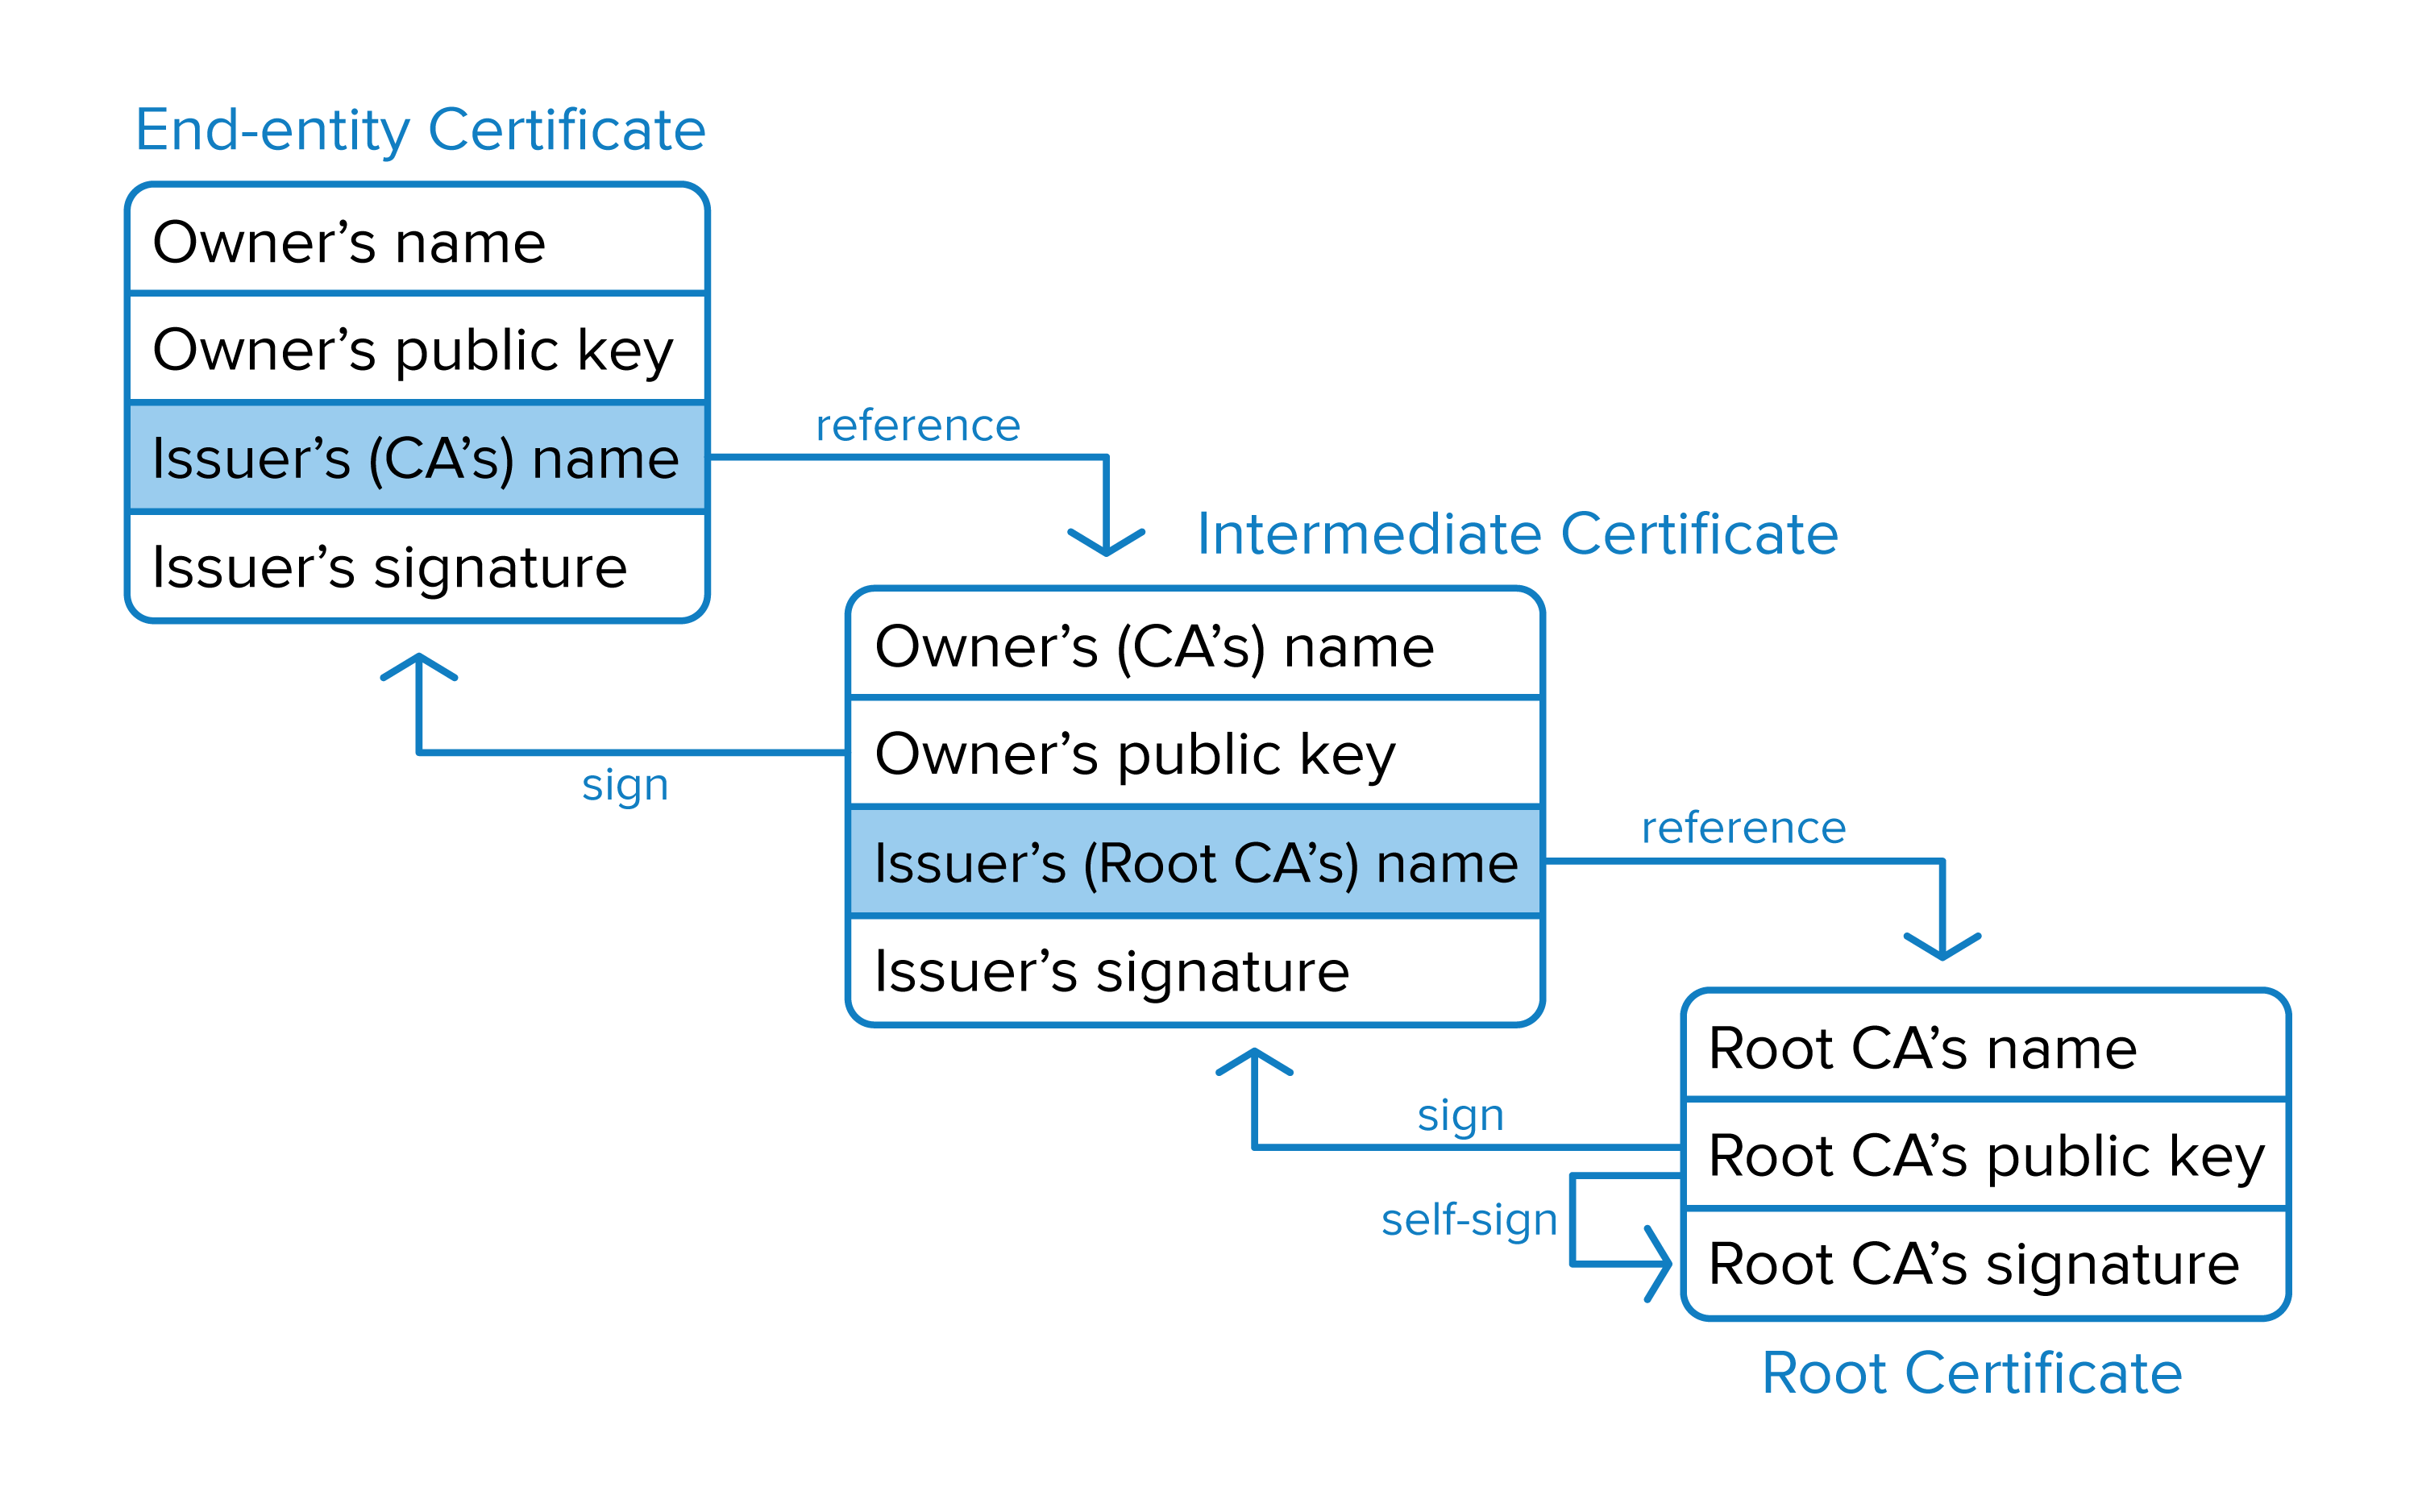
\includegraphics[width=0.8\textwidth]{images/tls-certificate-verification.png}
				\caption{TLS Certificate verification chain. \cite{image_tls_certificate_verification}}
				\label{fig:tls_certificate_verification}
			\end{figure}
			\par Usually certificates are bought by companies that wants to implement a secure connection with their clients. In this way the certificate obtained by the server is inserted in the tree of certificates, and every client can verify its authenticity. Note also that every machine can generate a self-signed certificate. What is indeed important is checking if the server certificate is linkable to a trusted Certificate Authority. \newline
			\par The Android operative system handles by itself a list of trusted certificates. These certificates belong to two categories: system certificates and user certificates. \newline
			\textit{System certificates} are used by default to verify all other certificates. So if we are using an application trying to connect to an application service, if the certificate obtained by the web service is traceable to one certificate already present in the system store, then the certificate is accepted and the connection is established. Notice that since the release of Android 7 Nougat, it is impossible to install any CA at system level without having root privileges on the device. \newline
			On the other way \textit{user certificates} are installable even at user level, and are used to verify certificates when directly expressed by the application.
			
		\subsection{Man-in-The-Middle}
		\label{subsec:mitm}
			\par \textbf{Man-In-The-Middle (MITM)} is an attack able to disrupt the security properties delivered by the TLS protocol. As the name suggests the attacker positions himself between the server and the client. The attacker acts like a proxy server intercepting every connection incoming from the client, pretending to be the real server, and forwarding them to the real server, pretending to be the real client. 
			\par On one side, at the moment of the TLS handshake, the client verifies the identity of the server, so the attacker needs to reproduce the handshake with the client in order to let it trust the attacker. As described in the last section, the authenticity check is performed through the exhibition of the server certificate. In this case the client needs to trust the certificate of the attacker. After having checked the identity of the server, the TLS handshake can continue following the standard procedure: client and attacker agree on a pre-master shared key and the encrypted communication will take place.
			\par On the other side the attacker needs to act as the real client for the server, so that every connection intercepted will be redirected to the server, and every response obtained will be delivered to the client. This is made possible by starting a new connection between attacker and server. The attacker will authenticate the server by checking its certificate and completing the standard TLS handshake with it. \newline
			At this point the attacker has performed two different TLS handshakes, one with the client faking to be the server, and one with the server faking to be the client. The man in the middle is now able to read messages sent or received from the client and forward or deliver them to the server. \newline
			\par A man-in-the-middle attack is what made possible the analysis of the communication protocol of every application I investigated. After having \textit{placed} ourselves inbetween client and server we will be able to understand what exactly is the protocol adopted by an android application and analyze each message looking for a possible leak detection of users personal data. For more specifics on how I performed a MitM attack for my case studies, read the chapter \textit{Testing Environments}, sections \textit{HttpToolkit}[Section \ref{sec:http_toolkit}] and \textit{BurpSuite}[Section \ref{sec:burp_suite}].
			
		\subsection{SSL Certificate Pinning}
			\par If the MitM attack results in the loss of authenticity in an HTTPS communication, the \textbf{SSL Certificate Pinning} is an hardening process that can be adopted in order to deliver an additional layer of security to the software. Pinning certificates or public keys is a countermeasure that allow web servers to control the risk of man-in-the-middle attacks or CA compromise. 
			\par The whole process of certificate verification described in the previous section is skipped, the application will indeed only validate certificates or public keys that are \textit{pinned} to the application. A MitM attacker will not be able to intercept messages anymore. The connection will be blocked right in the middle of client's and attacker's TLS handshake. The application implementing a certificate pinning method in fact will not trust anymore the attacker's certificate, and the connection will be dropped by the attacker's proxy.
			\par There are two ways of implementing this hardening technique. The first one is by \textit{preloading} the public key or certificate in the client at development time, so that every fake server trying to connect to the client is rejected during the TLS handshake phase. The second one happens at runtime by installing the \textit{pin} in the client once upon the connection is established by using the HTTP Public Key Pinning (HPKP) header, indicating the public key and the max age of validity for that specific pin. This second approach has been adopted by Chrome and Firefox for their browsers, but after some years new security issues has been discovered about it. Indeed in case of bad implementation (for example a pin of an incorrect public key) could bring to denial of service, but even in case of compromised server the consequences can be devastating for a longer time if HPKP is implemented, a bad pin might be established from an attacker that had the control of the server (HPKP Suicide~\cite{HPKP_suicide}). For this reason the public key pinning is now highly discouraged for web browsers. \newline
			\par In Android application SSL certificate pinning is a solution still able to protect from MitM attacks. The implementation is generally done by pinning a specific certificate inside the application logic at development time. There are multiple ways to implement a certificate pinning in Android as explained in \cite{android_ssl_pinning}. Among them two approaches can be identified: 
			\begin{enumerate}
				\item basing on \textit{Network Security Configuration}: A pretty simple certificate pinning implementation made possible by specifying a \textit{<domain-config> tag} in the network security configuration file present in the application. A \textit{pin-set} of \textit{pin} can be specified for the whole application.
				\item basing on the \textit{network library}: Many different network libraries exist for Android application (i.e. \textit{OkHttp}, \textit{Retrofit}, \textit{Volley}, and so on). Each one of them provide methods to skip the standard certificate validation procedure and implement the certificate pinning procedure.
			\end{enumerate}
			
		\subsection{Certificate Transparency}
		\label{subsec:certification_transparency}
			\par \textbf{Certificate Transparency} (CT) is a security standard adopted by browsers for monitoring and logging discrepancies in the certificate verification procedure. The whole system is manteined by a set of certificate logs handled by Certification Authorities and many browsers. These logs assume the form of \textit{Merkle trees} (also noticed as \textit{hash tree}), they are publicly verifiable, in append-only mode. The goal of this standard is to keep track of all valid certificates ever issued for a specific domain. \newline
			\par	This is the scenario: a domain owner implementing a web service requests a new certificate from a CA. Before releasing the new certificate, it submits the \textit{hash digest} of that certificate to one or more certificate logs, receiving a \textit{Signed Certificate Timestamp (SCT)} signed by the log provider. Once signed, the CA can now send back the certificate with embedded the SCT to the domain owner asking for the certificate. Every HTTPS connection to that web service will be served using that certificate. When a user wants to use the web service, browsers or mobile apps will query the trusted certificate log to find a record matching with the SCT of the certificate received by the web service. \newline
			\par In Android operative system, an example of application implementing the Certification Transparency mechanism is the Chrome browser. As we said above (see Certificate Verification [Section \ref{subsec:certificate_verification}]) Android certificates can be placed at system level or user level. Every application will use by default the system store to verify others certificates, and so does Chrome, if not specified differently. This application will choose whether to use the Certificate Transparency or not, basing on which store the certificate root is installed. When a certificate showed by any web service it is checked, if the root certificate met is present in the system certificates store then Chrome decides to also verify the Certificate Transparency requirement. On the other way if we are testing a web service showing a certificate that is inside the user certificates store, then the Certificate Transparency procedure is not applied.\newline 
			
	\section{Protocol Buffers}
	\label{sec:protocol_buffer}
		\par \textbf{Protocol Buffers}\cite{protocol_buffer}, also known as ProtoBuffers, are a language-neutral, platform-neutral extensible mechanism for serializing structured data. The development of this new mechanism started in the early 2001 from Google for private purposes. Then in the 2008 was publicly released as open-source data format. The design goal while developing Protocol Buffers was to provide a data serialization universal and faster then the standard XML. Nowadays it is widely used when an internaction between different architectures client-server is needed, that is the case for most of the Android application.
		\par The messages exchanged are data structures described in a proto definition file \textit{.proto}. After having compiled those definitions through \textit{protoc} they can be imported in any project written in the most used programming languages. Protobuf version 2.0 was providing a code generator compatible with \textit{C++}, \textit{Java}, \textit{C\#} and \textit{Python}. The version 3.0 extended the programming language compatibility also to \textit{Go}, \textit{Ruby}, \textit{Objective-C}. Other languages are supported through third-party implementations (\textit{C},\textit{JavaScript}, \textit{Perl}, \textit{PHP}, \textit{Scala}). 
		\par To give an idea on how the mechanism works, let's say a client-server application would like to serialize data about a \textit{Person}. In order to let both endpoint to know about the data structure \textit{Person}, both of them require to integrate in their project that data structure. The definition of \textit{Person} is done in a \textit{.proto} file:
\begin{lstlisting}
message Person {
	optional string name = 1;
	optional string email = 2;
	optional string phone = 3;
}
\end{lstlisting}	
		The proto file has to be done only once, and it is independent from the platform we will be using. To import the definition of the above \textit{Person} data structure in our project we need to run the \textit{protoc} compiler obtaining the ready-to-use structure. \newline
		\par Since the native language for Android application is Java, running \textit{protoc} we are interested in the \textit{.java} classes generated. For each message type defined in the \textit{.proto} file will result a couple of \textit{.java} files: one will contain the definition of the object itself, the other one is the Builder for that specific object type. The first one will be provided of the standard accessor's methods (in our case \textit{hasName()}, \textit{getName()}, and so on for each field), while the second one will have both getters and setters methods (\textit{getName()}, \textit{setName()}, and so on for each field). At this point it is needed to import those definitions in \textit{.java} classes thanks to the Protocol Buffer API provided by the mechanism itself. This is a picture summarizing the whole procedure:\newline
		\begin{figure}[ht]
				\centering
				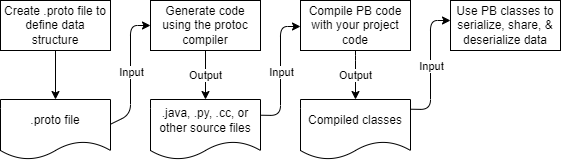
\includegraphics[width=0.9\textwidth]{images/protobuffer.png}
				\caption{Procol Buffer workflow \cite{protocol_buffer}}
		\end{figure}
		\par Each object already instantiated is immutable, it can only be modified through its respective Builder methods at the moment of its building. The procedure to instantiate a new \textit{Person} object in the application is respectively: 
		\begin{enumerate}
			\item Contruct a builder for the object. 
			\item Set any field to any acceptable value.
			\item Call the builder's \textit{build()} method.
		\end{enumerate}
		\par In particular the step 2 is made possible through the mehods provided automatically in those \textit{.java} files. Each one of them will modify the structure created at step 1, and it will return a new \textit{Builder} object, such that it can be repeatedly modified and at the end instantiated through the \textit{build()} method. \newline
		\par The above defined \textit{Person} class, it is just an example. The Protocol Buffer mechanism is able to provide a platform-independant really complex classes with repeated fields, nested classes, constant values or even rpc services to define. At the same time the use of Protocol Buffer let the developer save time  when developing the data structures. Indeed the \textit{.proto} definition has to be done only once, and it is valid for every kind of platform that would use that type of structure.

	\section{gRPC}
		\par \textbf{gRPC} \cite{grpc} is a cross-platform \textit{Remote Procedure Call} (RPC) framework. The mechanism was initially created by Google for private purposes, but in 2016 it was publicly released as open-source. As a remote procedure call framework, it let the developer to define in an application some methods that will actually run on a different machine from the one running the application. Generally the idea behind any RPC system is to define a \textit{service} able to execute a specific method in order to call it remotely from any another application.
		\begin{figure}[ht]
			\centering
			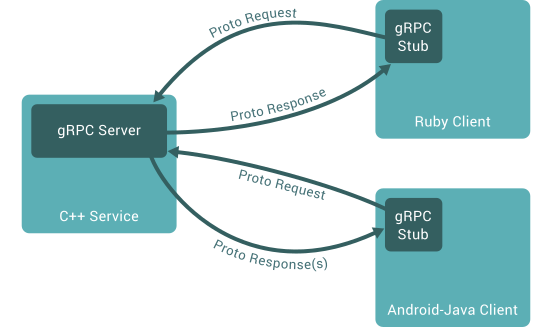
\includegraphics[width=0.7\textwidth]{images/grpc.png}
			\caption{gRPC workflow \cite{grpc}}
		\end{figure}		
		\par What makes gRPC so powerful is the fact it is based on \textit{HTTP/2} protocol for the transport layer, and uses \textit{Protocol Buffers} (described in Section \ref{sec:protocol_buffer}) as its Interface Description Language (IDL). The combination of these two mechanism let the gRPC system to provide an easy access and platform independant solution for the implementation of a RPC system. \newline
		In a gRPC system, as any other RPC system, we can differentiate between \textit{gRPC Server} and \textit{gRPC Stub}, the part of the client implementing the gRPC framework. On the server side, the server implements the interface for the specific method it is able to execute, and handles the incoming client calls. On the client side, the gRPC Stub provides the same method as defined by the server. What really happens in the moment in which the client invoke the method is that:
		\begin{enumerate}
			\item The gRPC Stub serializes the parameters passed to the method using the Protocol Buffer mechanism. Then sends over an HTTP/2 connection the method request together with the serialized data.
			\item The gRPC Server accepts the incoming request from the client and deserializes the data using the Protocol Buffer mechanism.
			\item The gRPC Server will execute the method specified by the client.
			\item Once the result is available, the gRPC Server sends over the HTTP/2 connection the response containing the return value for that specific method, serialized with the Protocol Buffer mechanism.
			\item The gRPC Client deserializes the return value using the Protocol Buffer mechanism.
		\end{enumerate}
		\par Even if different IDLs can be specified while defining the gRPC service, JSON for example, by default the gRPC framework uses Protocol Buffers. Moreover the framework provides features like \textit{authentication} (through TLS or token-based authentication) and \textit{bidirectional streaming}.
		
	\newpage
	\section{QUIC}
		\par \textbf{QUIC} is a general-purpose transport layer network protocol designed by Google. It was publicly announced in 2013 and after some years under the experimental state, in the recent 2021 became a standard as defined from the Internet Engineering Task Force (IETF) in \textit{RFC 9000} \cite{rfc9000}.\newline
		\par The main goal of QUIC is to improve the performance of the connection-oriented web applications, that for years have been run basing on TCP as transport layer network protocol. QUIC establishes a number of multiplexed connections using UDP instead, allowing multiple streams of data to reach different endpoints independently. The same concept is possible in HTTP/2 with multiplexed connections, but what really suffers this last one is the the head-of-line-blocking delays related to the connection-oriented TCP which it relies on. \newline
		\par Briefly the \textit{Head-of-Line blocking} (HOL blocking) is an issued generally affecting every packet that need to pass through a line. If the First-In-First-Out (FIFO) method is used, the longer the packet has arrived in the queue, the higher is the priority it has to be sent over the line. With the release of HTTP/2, this issue was partially resolved through the multiplexing of multiple connection, letting multiple HTTP requests running together but still an implementation over a single TCP connection. If one packet is being lost in the transmission than the whole connection will be waiting for the retransmission of that single packet. Now in the case of a client with few connections towards a bunch of server is waiting time is neglactable, but modern Android applications are implementing different services at the same application, using both standard HTTPS requests and gRPCs with an high number of structures to serialize through Protocol Buffer towards hundreds of endpoints. In case of a packet retransmittion the performance loss will be evident.
		\par QUIC protocol addresses this issue by relying on \textit{UDP} as transport layer protocol. UDP is a connectionless transport layer protocol without any implementation of packet orderding and retransmission, indeed every packet is forwarded to the endpoint individually, without any risk of HOL blocking problem. At the same time UDP does not provide any guarantee on the packets delivery making the whole connection unreliable. All  these checks are in fact implemented in QUIC on top of UDP, while still taking advantage of the performances achieved by UDP. Every additional connection feature, like TLS encryption, is done in the same way on top of UDP. \newline
		\par The second goal of QUIC is to improve the connection latency between the two endpoints. Using UDP as transport layer protocol the TCP overhead needed for the connection management is already cutted off. Most of the applications will demand for TLS encryption requiring its own handshake, that would be summed up to the TCP three way handshake if using the HTTP/2 protocol. With QUIC there is no redundancy in those handshake phases. It is done only once in QUIC as showed below:
		\newline
		\begin{figure}[ht]
			\centering
			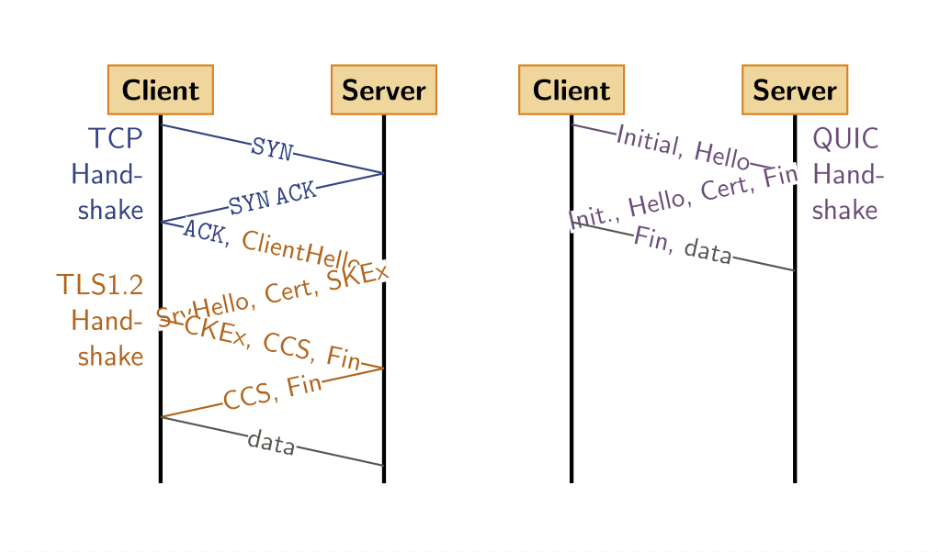
\includegraphics[width=0.8\textwidth]{images/quic_handshake.png}
			\caption{Comparison between TCP+HTTPS and QUIC handshakes}
		\end{figure}	
		\par Moreover, as said above, UDP does not handle loss recovery, meaning that QUIC is also resposible for each separated controlled flow. Others improvement in terms of overall latency are adopted, for example packets are individually encrypted, so that can not result in a waiting for partial packet.\newline
		\par Another property of QUIC is the ability to mantain its performance during network-switch events that frequently happens in mobile devices, like the connection transition between WiFi hotspot and mobile network. In HTTP/2, based on TCP, every connection is timed-out one by one and then re-established on the new network, while in QUIC at every connection is assigned an identifier that is kept even if the source ip address changes.
		\par Lastly, QUIC is completely handled at application level. There are numerous libraries available in order to implement this protocol in an application: \textit{Cronet} developed by Google, \textit{sn2-quic} developed by Amazon Web Services, \textit{proxygen} by Facebook and so on.\newline
		For a practical example see the application case Google Maps in Section \ref{sec:google_maps}.
	
		
		\subsection{HTTP/3}
			\par In June 2022 the IETF published \textbf{HTTP/3} as the major version of the \textit{HyperText Transfer Protocol} in \textit{RFC 9114}\cite{rfc9114}. Unlike the earlier versions of HTTP 1.1 and 2.0 based on TCP, HTTP/3 relies on QUIC, based on UDP. \newline
			\par HTTP/3 uses the same semantics of the previous versions (request methods, status codes, message fields) but it differs in the way it mantains the connection session. Most of the changes in HTTP/3 are in the way the protocol interfaces with the underlaying transport layer. The new version of HTTP results in lower latencies and higher performance in real-world usage, mostly due to the adoption of QUIC. 

		\chapter{Testing Environment}
\label{chap:testing_environment}
	
	\par In this chapter is described the whole environment where I settled the investigation of each Android mobile application discussed in this thesis.
	\par Core of the environment is the \textit{Android Studio} framework, offering both an Integrated Development Environment (IDE) and testing features for Android mobile applications. Here I configured an emulated device where I could run the application cases I investigated.
	\par Once installed the specific application I had to analyze the \textit{network traffic} generated by itself. Generally it is rare a single tool is perfect for all the applications to analyze, this is the reason why I used different tools to inspect the network traffic generated by an application, instead of just sticking with one tool. Starting from the standard-de-facto in packet inspection \textit{Wireshark} program, ending to tools acting like proxy servers between the client application and the server. Some of these tools are able to automatically install and configure a man (MitM attack [\ref{subsec:mitm}]) in the middle of the communication, others might need some manually configuration. \newline
	The whole amount of informations exchanged between application and server is hidden somewhere in the communication. It might be more or less difficult to find them, but all the informations are there, in those packets.
	\par Other tools revealed to be aswell useful while investigating Android applications. Dynamic instrumentations tools are softwares able to run scripts from the inside of the applicaiton, as they were part of it. At the same time, static analysis tools provided informations on class and libraries used by the application, simply basing on source code of the application itself.
	
	\section{Android Studio}
		\par \textbf{Android Studio} is the center of the testing environment. Other than a complex IDE software, it provides a complete testing suite for Android mobile applications. Once installed the software, it enables the access to the Android Device Manager tool, where the user can create an emulator for a specific Android device choosing among phones, tablets, wearOS or TVs. 
		In this section I will explain how I prepared the android virtual device in order to obtain a working environment that made possible the application investigation.
		
		\subsection{Android Virtual Device (AVD)}
			For my purpose study case I created an \textit{Android Virtual Device} (AVD) phone with the same properties of the \textit{Pixel 3a} phone developed by Google, that is \textit{5.6''} screen size, \textit{1080x2220} resolution, \textit{440dpi} density. The device is running \textit{Android 13}, also known as \textit{Tiramisu} version, or \textit{API 33}, on \textit{x86\_64} architecture. In the really first step while selecting the hardware we would like to use for the virtual device, some device definitions are enabled to run the Play Store software, and so it is for our Pixel 3a device. This is really useful since I had not to download and install manually each applications on the device. Indeed it is made possible using the Google Play store directly from the emulated device. 
			\par Once created the new virtual device (in my case called \textit{''Pixel\_3a\_API\_33\_-\_Data\_Leak\_Detection''}), it is possible to run it through the Android Device Manager. For simplicity I created a simple \textit{.bat} file to run the virtual device without the need to open Android Studio everytime. Indeed there is a file called \textit{emulator.exe} in a the folder where we installed the Android SDK. We can simply open the emulator by command line passing the name of our AVD and some optional arguments. Here it is how my command looks like:
\begin{lstlisting}[language=bash, caption={run\_AVD.bat}]
C:\<Android_folder>\Sdk\emulator\emulator -feature -Vulkan -memory 2048 -netdelay none -netspeed full -avd Pixel_3a_API_33_-_Data_Leak_Detection
\end{lstlisting}
		\par More specifically the \textit{-feature -Vulkan} argument will force the emulator to do not use the \textit{Vulkan} graphic library. Since Android API 30 lots of android applications, such as Google Chrome, use this library to boost its performance. Anyway in some devices, especially for the emulated ones, might result in a massive slow rendering time. Other arguments are specifying to dedicate 2 Gb of RAM memory for the device, to not impose limits on the network speed and to not simulate any network delay.
			\par Here there is the full property list of the device I used:
			\begin{center}
				\begin{tabular}{ |p{5cm}||p{9cm}| }
					 \hline
					 \multicolumn{2}{|c|}{Android Virtual Device (AVD) Properties} \\
					 \hline
					 \hline
					 avd.ini.displayname & Pixel 3a API 33 - Data Leak Detection \\
					 AvdId & Pixel\_3a\_API\_33\_-\_Data\_Leak\_Detection \\
					 image.androidVersion.api & 33 \\
					 image.sysdir.1 & system-images/android-33/google\_apis\_playstore/x86\_64/ \\
					 tag.id & google\_apis\_playstore \\
					 hw.device.name & pixel\_3a \\
					 hw.device.manufacturer & Google \\
					 hw.cpu.ncore & 4 \\
					 hw.ramSize & 1536 \\
					 vm.heapSize & 228 \\
					 hw.lcd.width & 1080 \\
					 hw.lcd.height & 2220 \\
					 hw.gpu.enabled & yes \\
					 hw.gps & yes \\					 
					 hw.accelerometer & yes \\
					 runtime.network.speed & full\\
					 runtime.network.latency & none \\
					 \hline
				\end{tabular}
			\end{center}

			%\begin{figure}[!ht]    
				%\centering   
				%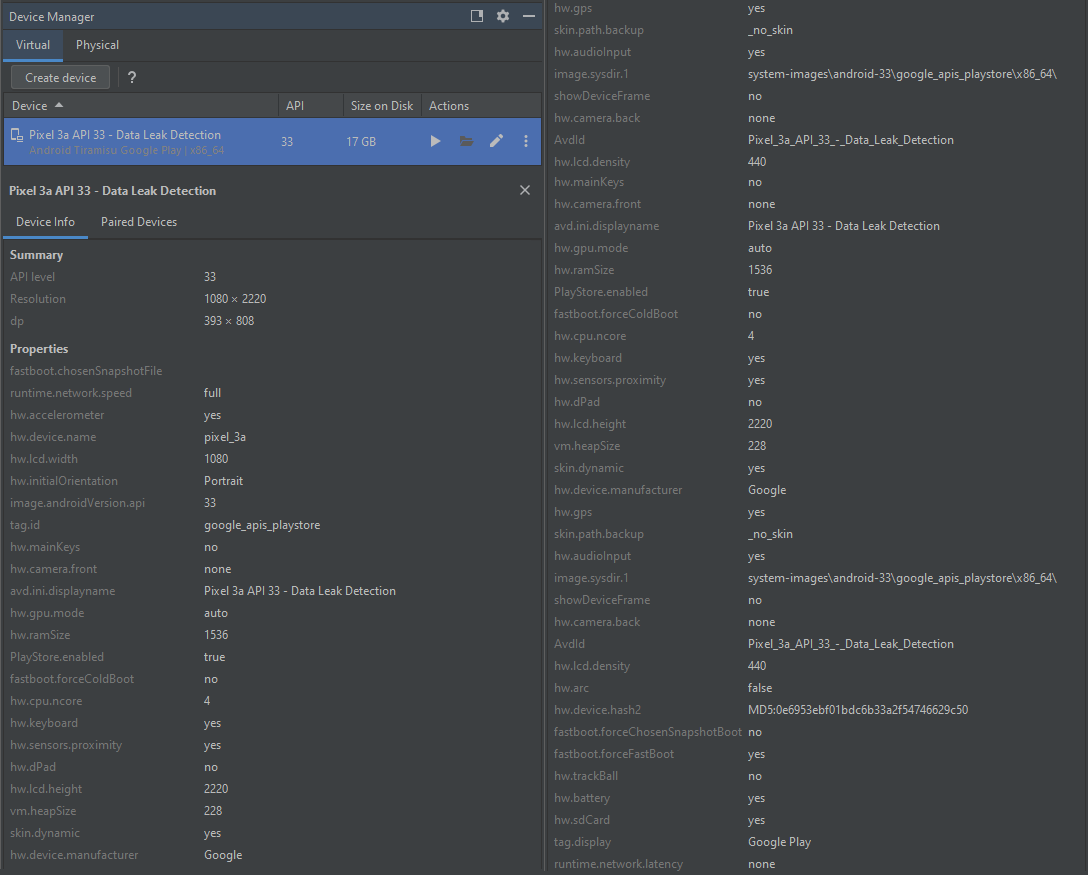
\includegraphics[width=0.9\textwidth]{./images/avd_splitted.png}
			    	%\caption{Android Virtual Device (AVD) specifics}
			%\end{figure}
			
		\subsection{Root privileges on virtual device}
			\par After having succesfully created the AVD, it can result useful to get the \textit{root privileges} on the device. In our case it is really mandatory since what we are going to do is intercept the communication protocol in the middle between application and server. As explained in the Section \ref{subsec:mitm}, the client application needs to trust the proxy server, and this is done by checking its certificate. Starting from the release of version \textit{Nougat} (API $\ge$ 24), of Android operative system, it changed the behaviour adopted by android applications in trusting users. If before the application was checking both \textit{user certificates} and \textit{system certificates}, now it will check exclusively the installed system level certificates, therefore root privileges are mandatory. \newline
			\par There are so many tools that let a user obtain the root privileges on his phone. I personally have used the \textit{rootAVD} tool available online \cite{rootAVD}. The procedure is really simple, firstly run the command with argument \textit{ListAllAVDs} to list all the AVDs on the machine. We will obtain the full path of our AVDs, that we will pass as argument when executing the tool from command line. The tool will make use the \textit{adb} tool that Android Studio brings together with its development tools, so it is worth it to explain what it is.
		
		\subsection{Android Debug Bridge (adb)}
			\par As I said Android Studio offers a complete set of features to run and test android application. In particular by installing the \textit{Android SDK Platform Tools} package from Android Studio, we will obtain a set of tools that make possible the debug of our application. \newline
			One of the most important tools is the Android Debug Bridge, more noticed as \textit{adb}. It is a command line tool that let the user directly communicate with an Android device, let it be a physical or emulated device. Basically it is a client-server program that runs both on our machine and Android device. There is then a client, that is the command line tool, a daemon \textit{adbd} running in the background of the Android device, and a server managing the connection between client and daemon. For a complete understanding of the adb tool check the Android Developer guide \cite{adb}.
		
	\section{Network traffic analysis}
		\par Once the virtual device is well configured as described above, let's start introducing some network tool I used for my study cases. Each one of them has some strengths, one tool might works for an application but not work for another. They are listed below in order of complexity. \textit{HttpToolkit} and \textit{BurpSuite} are network traffic interceptors, that means every connection outgoing from our device will be intercepted by these applications, letting the user to inspect more or less accurately how the request were formed. \textit{Wireshark} on the other way is a packet sniffing tool, meaning that it will capture any packet in the network, regardless of the protocol or the port used. 
		
		\subsection{HttpToolkit}
		\label{sec:http_toolkit}
			\par HttpToolkit\cite{http_toolkit} is an open-source tool for debugging, testing and building with HTTP(S). The strength of this tool relies on its simplicity for configuring the environment. Once downloaded the application it requires to be connected to a source of traffic. HttpToolkit provides a variety of available sources, from the most famous browser (Chrome, Firefox, Safari, Edge), up to more complicated environment, such as Docker containers, virtual machines, Android devices or iOS devices. In this case the network source to monitor is the Android virtual device where the applications will run. The program itself will notify the user which are the available sources of traffic at the start up. Since the scope of the study is investigating applications running on the android emulator, it is needed to download from Google Play the HttpToolkit application also on the virtual device. Once installed the android app, the HttpToolkit running on the computer will automatically notice the new source called \textit{''Android device via ADB''}. Just click on it and the whole proxy system is automatically configured. \newline
			\par In this phase it is crucial to understand what is happening:
			\begin{itemize}
				\item HttpToolkit will inject a custom certificate on our device, communicating with it through ADB. Since we also have the root privileges on the android emulator, the certificate willl be placed in the folder of the \textit{System Certificates} that is \textit{/system/etc/security/cacerts} in the Android device. \newline
				\item The respective HttpToolkit Android application will be activated in order to set up a VPN, redirecting the whole network traffic directly via the Android Debug Bridge to the main HttpToolkit program running on the computer. \newline
				\item HttpToolkit will copy to the device, again via ADB, a file containing the command used to start up the Android Google Chrome application. 
\begin{lstlisting}
chrome --ignore-certificate-errors-spki-list=<hash_digest>
\end{lstlisting}
This specific command will bypass the Certification Transparency check described in the section \ref{subsec:certification_transparency}. The command looks like the following, where \textit{hash\_digest} is the hash digest of the SSL certificate used by the tool.\newline
			\end{itemize} 
			
			\par All these steps are done automatically from the program itself. Indeed this tool requires almost no configuration on the user side, aside from the preparation of the AVD discussed in the above section.
			\par	As described in the certificate verification [Section \ref{subsec:certificate_verification}] and MiTM [Section \ref{subsec:mitm}], this is the moment in which the HTTP(S) requests outgoing from the application case are intercepted by HttpToolkit, showing precisely each request detail. Then they are forwarded to the application server. Same happens for the HTTP(S) responses. Moreover in case certificate is rejected by the application, that means some certificate pinning procedure has been adopted, the tool will notify us.
			\par Anyway HttpToolkit is only able to intercept the HTTP(S) protocol, that is enough for most of the Android applications. In case the application will communicate in a different protocol (QUIC for example) the requests are not visible to this tool, so we will need a different network tool.
		
		\subsection{BurpSuite}
		\label{sec:burp_suite}
			\par \textbf{Burp Suite} is one of the most famous web security suite. It is available in different versions: \textit{Community Edition}, \textit{Professional Edition} and \textit{Enterprise Edition}. The first one is more than enough for personal and research purposes and it is the one I used. It contains the essential toolkit letting the user to be able to set up a proxy and perform a MiTM interception while analyzing the content of the requests passing through the proxy. Differently from HttpToolkit it is more flexible in terms of protocols able to intercept, for example HTTP/3 over QUIC, and it is way more customizable. Indeed it let the user set up specific listeners (address and port), or import/export specific CA certificates with which decode the encrypted messages. Moreover it provide a specific \textit{''Repeater''} tab where the user can manually craft or modify already existing requests and forward them to the endpoint. This last one feature is a routine very useful that I used for every application case.
			\par On the other side, this tool is not auto-configured to intercept traffic coming from mobile device. Everything has to be manually set on both proxy side and mobile device side. Theoretically the configuration steps to enable the interception of HTTPS requests are the same described in the previous section, that HttpToolkit was doing automatically, but instead in this case have to be applied manually \cite{burp_suite}:
			\begin{itemize}
				\item From the Proxy options, export the CA certificate in \textit{DER format}. This is the certificate that we will manually have to install as system-level in the Android operative system. Anyway Android will read only a \textit{PEM format} certificate. Once exported the certificate we will need to convert the certificate using the \textit{openssl} tool available for every platform. But this is not enough, in fact the certificate needs to have the filename equal to the \textit{subject\_hash\_old} value (that is the \textit{hash} of the certificate subject name computed by OpenSSL with the \textit{''old''} version 1.0) appended with \textit{0}. The command lines to achieve the result are:
\begin{lstlisting}
$ openssl x509 -inform DER -in <cacert>.der -out <cacert>.pem
$ openssl x509 -inform PEM -subject_hash_old -in <cacert>.pem | head -1
$ mv cacert.pem <hash_digest>.0
\end{lstlisting}
				This certificate has to be pushed to the device, and then moved to the \textit{/system/etc/security/cacerts/} folder, modifying its permissions. Notice that the ADB tool cannot execute commands as root user while using \textit{play\_store} images of Android (kernel images builtin with Google Play application) as in our case. Firstly it has to be pushed on the \textit{/sdcard/} location and than moved with the \textit{adb shell -c ''mv <source> <dest>''}:
\begin{lstlisting}
$ adb push <hash_digest>.0 /sdcard/
$ adb shell su -c ''mv /sdcard/<hash_digest>.0 /system/etc/security/cacerts/''
$ adb shell su -c ''chmod 644 /system/etc/security/cacerts/<hash_digest>.0''
\end{lstlisting}
				Be aware that rebooting the device will remove the certificate and the procedure has to be done again.\newline
				\item From Proxy options, we have to set up the correct listener. In our case we manually insert the specific IP address of our machine (since the traffic generated from the emulator will have that IP address) or just we can select \textit{All interfaces}. The port can be anyone available, let it be \textit{8082}. Respectively on the Android emulator we have to redirect the outgoing traffic to that proxy. A common proxy setting in the WiFi connection is fine: the IP address will be the one of the computer running Burp Suite, the port will be \textit{8082}.\newline
				\item Lastly we will have to fix the Chrome behaviour on the application in order to do not apply Certificate Transparency for that specific certificate. In any case this step is optional since we will not be using Chrome, but the Android application itself.\newline
			\end{itemize} 
			\par After having configured Burp Suite in this way, by clicking on the \textit{Intercept is off} in the \textit{Proxy} tab, we will be able to intercept any request outgoing from the Android emulated device. As well we can consult the HTTP history of the requests. More than this, we can click \textit{Send to Repeater} from a specific request to manually edit the fields, like Headers or Body, and forward it to the endpoint.
		
		\subsection{Wireshark}
		\label{sec:wireshark}
			\par \textbf{Wireshark} is the most famous packet sniffer tool. Differently from the two tools described before, Wireshark is a low level network protocol analyzer meaning that every packet outgoing from the selected Network Card Interface will be captured being able to analyze them. This tool will not differentiate between protocols, every packet will be captured. \newline
			\par Wireshark is a really powerful tool, also able to decrypt TLS communications if provided with the so called \textit{pre-master secret key}. This step is easily possible on Windows, Mac, or Linux operative system by setting an environment variable, so that the browser is enabled to export the secret key used in their encrypted communication. Once exported the pre-master shared keys, it is possible to instruct Wireshark to decode the TLS traffic by using those secret keys. Anyway this is not possible in Android operative system, or at least in this way. In fact it is possible to extract pre-master secret key used by a specific application with Frida. See Application Cases (Section \ref{use_cases}for practical examples) \newline
			\par Another possible approach in order inspect decrypted TLS communication in Wireshark is by using some other proxy tool capturing the network traffic at proxy level and capable of exporting the packet logs in \textit{.pcap} or \textit{.pcapng} format. Then is possible to open those logs with Wireshark and analyze every packet captured by the proxy.
			\par In this study Wireshark has been used complementarily to the previous tools HttpToolkit and BurpSuite. In particular since it captures any type of communication protocol, I used Wireshark to know if the Android application was adopting a network protocol different from HTTP(S) or QUIC, and in case I analyze that one.
	
	\section{Dynamic instrumentation}
	\par \textit{Instrumentation} is a concept of computer programming in which a user obtain informations, or generally trace and profile the behaviour of a software at runtime execution. Specifically \textbf{Dynamic instrumentation} tools are able to inject user scripts in the really first phase while running the target application. The injected script is user-defined such that library calls or specific functions can be traced at runtime execution. For this study I used two dynamic instrumentation tools compatible with the Android environment, that are \textit{Frida} and \textit{Objection}.
	
		\subsection{Frida}
			\par \textit{Frida} is a dynamic code instrumentation toolkit. Frida let the user inject user-defined scripts into native applications running on \textit{Windows},\textit{MacOS}, \textit{GNU/Linux}, \textit{iOS}, \textit{watchOS}, \textit{tvOS},\textit{Android}, \textit{FreeBSD}, and \textit{QNX}. This tool is written in \textit{C} language and basically it injects the \textit{QuickJS} JavaScript engine in the target process. This engine will execute the user-defined \textit{JavaScript} script with full access to memory and functions inside the process. One of the strengths of this tool, aside from its extreme compatibility with so many operative system, is the fact that the \textit{JavaScript} script can directly handle \textit{Java} classes and methods because of the use of Java bridge. So for example in the script we can directly intercept the Java contructs and modify their behaviour. 
			\par The installation is pretty simple and can be done via PyPI. The downloaded tool will be the client that we directly use from command line. In fact, since the study deals with Android application, we will need another component of Frida running inside the Android environment, that is \textit{frida-server}. Once downloaded this component will be placed on the Android emulator and get it started. Both \textit{frida-tools} (the client on the host machine) and \textit{frida-server} (the deamon running on the Android device) are able to communicate via ADB. Notice that root permissions are required on the Android device.
			\par There are two ways of injecting scripts in a target Android application:
			\begin{itemize}
				\item The first way is the immediate one. Just write your script in \textit{JavaScript} and let the \textit{frida-tool} inject it into the target application:
\begin{lstlisting}
$ frida -U -l <script.js> -f <andoid.package>
\end{lstlisting}
				The \textit{-U} argument specifies to Frida to interact with the USB device (Android emulator via ADB).\newline
				The \textit{-l <script.js>} argument specifies to load the user-defined \textit{script.js}.\newline
				The \textit{-f <android.package>} argument specifies the target Android application. The application wil be spawned and instantly frozen, the script injection takes place, and the application is then resumed.  
				\item The second way by using the Python API for Frida. The user creates a Python script which will directly handle the Frida injection in its script. Here there is a simple example:
\begin{lstlisting}
import frida, sys

jscode = ''''''
	Java.perform(() => {
	
	})
''''''

process = frida.get_usb_device().attach('<android_package>')
script = process.create_script(jscode)
print('[*] Running Android Application')
script.load()
sys.stdin.read()
\end{lstlisting}
			The Android process is selected by \textit{frida.get\_usb\_device().attach()} method.
			The script is a python string containing a \textit{Java.perform(() =>\{\})} function, and it is loaded with the \textit{process.create\_script()} method.
			The script is then load into the process with the \textit{script.load()} method.
			\end{itemize}
			\par The Frida toolkit comes embedded with some useful tools like \textit{frida-ps} and \textit{frida-trace}, letting the user respectively to check which process is running on the Android device, and to trace library calls while running a specific Android application. For more details check the Frida Documentation\cite{frida}. \newline
			For specific use cases check the Application Case (Section \ref{chap:use_cases}).

		\subsection{Objection}
		
	\section{Static analysis}
		\subsection{GDA}

		\chapter{Application cases}
\label{chap:use_cases}
	\par This chapter deals with every application case discussed in the study. As I explained three different area of interest mobile applications have been investigated: \textit{Weather}, \textit{Health \& Fitness} and \textit{Maps \& Navigation}. The application case sequence choice  has been made by following an increasing complexity order and an increasing amount of informations exchanged. \newline
	\par Generally the applications belonging to the first category do not require any form of user authentications, meaning that few private informations would be shared about the user. For this reason a single application has been taken under examination, that is \textit{iLMeteo}.\newline
	The application that falls in the second category, often have an higher degree of customization in terms of user profile, also implementing some features for user interaction in the application logic. This is the case of \textit{Pacer}, in which the investigation brought some really interesting results.\newline
	The last category is potentially the highest source of private user informations retrievable. Maps and Navigator applications require a continuous data exchange between client and server, in oder to deliver specific real time features, like the computation of the fastest path or the current traffic situation. Three different application have been taken in considerations, that are \textit{RadarBot}, \textit{Waze} and \textit{GoogleMaps}. \newline
	Obviously the higher the competitor is, the higher the analysis would be harder. This is the reason why there are so many concepts explained in the Fundamentals chapter (Section \ref{fundamentals}). Most of them are used not only to improve the application performance, but also to harden the security of the application itself. \newline
	\par The research study conducted application by application is reported in the following sections.
	
	\section{Application case: iLMeteo}
		\par Descrizione
		\subsection{Study detail}
			\par 
		\subsection{Sensitive data}
		\subsection{Other vulnerabilities}

	\section{Application case: Pacer}
	\label{sec:pacer}
		\subsection{Study detail}
		\subsection{Sensitive data}
		\subsection{Other vulnerabilities}
		
	\section{Application case: RadarBot}
		\subsection{Study detail}
		\subsection{Sensitive data}
		\subsection{Other vulnerabilities}

	\section{Application case: Waze}
		\subsection{Study detail}
		\subsection{Sensitive data}
		\subsection{Other vulnerabilities}

	\section{Application case: GoogleMaps}
	\label{sec:google_maps}
		\subsection{Study detail}
		\subsection{Sensitive data}
		\subsection{Other vulnerabilities}
		\chapter{Conclusion}
	

	\backmatter

		\cleardoublepage
		\phantomsection
		\addcontentsline{toc}{chapter}{\bibname}
		
		\begin{thebibliography}{99}
			\bibitem{European Commission} European Commission - What is personal data \newline
			\url{https://commission.europa.eu/law/law-topic/data-protection/reform/what-personal-data_en}
			\bibitem{android_dev_tips} Android Developers - Security with network protocols \newline
			\url{https://developer.android.com/training/articles/security-ssl}
			\bibitem{image_tcp_tls_handshake} Cloudflare - TLS Handshake \newline
			\url{https://www.cloudflare.com/it-it/learning/ssl/what-happens-in-a-tls-handshake/}
			\bibitem{image_tls_certificate_verification} Okta Developer - Certificate Validation \newline
			\url{https://developer.okta.com/books/api-security/tls/certificate-verification/#tls-certificate-verification}	
			\bibitem{certificate_pinning} Digicert - What is certificate pinning \newline
			\url{https://digicert.com/blog/certificate-pinning-what-is-certificate-pinning}				
			\bibitem{HPKP_suicide} Scotthelme.co.uk - Using security features to do bad things \newline
			\url{https://scotthelme.co.uk/using-security-features-to-do-bad-things/}
			\bibitem{android_ssl_pinning} Appmattus Medium - Android Security SSL Pinning \newline
			\url{https://appmattus.medium.com/android-security-ssl-pinning-1db8acb6621e}	
			\bibitem{rootAVD} GitHub - rootAVD \newline
			\url{https://github.com/newbit1/rootAVD}
			\bibitem{adb} Android Developers - Android Debug Bridge \newline
			\url{https://developer.android.com/studio/command-line/adb}
			\bibitem{http_toolkit} Http Toolkit - Docs \newline
			\url{https://httptoolkit.com/docs/}
				

		\end{thebibliography}

\end{document}


